\chapter{Short duration conditions: diarrheal diseases}
\label{applications-short_dur}

The next two chapters consider the application of this framework to
conditions where data on incidence is found in systematic review but
direct measurement of disease prevalence is done rarely.  This is the
case with acute conditions that have duration on the order of days or
weeks, such as diarrheal disease.  Since the incident event in this
diseases is the source of the measured data, it is much more common to
find a study on how many incident cases were observed during a period
of time than how many prevalent cases there were at any instant.  It
is estimates of prevalence that are needed for the GBD 2010 Study to
estimate disease burden, however.  The compartmental model, together
with assumptions on the duration of disease provides a mechanism for
estimating prevalence from incidence data, and investigating this is
the topic of this chapter.

Diarrheal diseases are a leading cause of childhood morbidity and
mortality.  Typically defined as having loose or watery stools three
or more times a day or more frequently than normal for the individual,
the diarrheal episodes typically last 1-8 days for acute cases
depending on severity. \cite{unicef_diarrhoea_2009,
  carlos_etiology_1990, lamberti_systematic_2012} Compared to many of
the other diseases discussed thus far, diarrheal diseases have a very
short duration.

Bacterial, viral and parasitic infections cause most cases of
intestinal infectious diarrhea.  Typically spread via the oral-fecal
route, water sanitation and hygiene are a large part of diarrhea
prevention.  Treatment usually involves fluid replacement, as acute
diarrhea causes fluid loss and dehydration.  Common prevention
strategies include vitamin A and zinc supplementation, vaccinations
and antibiotic regimes. \cite{wardlaw_diarrhoea:_2010,
  carlos_etiology_1990, lamberti_systematic_2012}

For the analysis of diarrheal diseases, the primary sources of data
are from surveys, hospital admissions and literature review.  The
surveys report period prevalence data whereas hospital admissions and
the majority of the literature report incidence data.  In short term
diseases, point prevalence is approximately the same as the product of
incidence and disease duration.  Therefore to avoid compositional
bias, all incidence and period prevalence estimates were converted to
point prevalence estimates using the assumption that
    \begin{equation}
    	h_{p_{point}}=h_{p_{period}} *
        \frac{h_{d}}{h_{d}-1+X_{recall}}
    \end{equation}
where $h_{p_{point}}$ is the point prevalence, $X_{recall}$ is the
survey recall period and $h_{d}$ is the mean duration of the disease.
Thus the analysis includes 2029 rows of prevalence data from 19
regions.  Data from Central Latin America is shown in Figure
\ref{fig:app-diarrhea data}.  Cause-specific mortality assumes that
anyone with the disease died of the disease.

    \begin{figure}[h]
        \begin{center}
            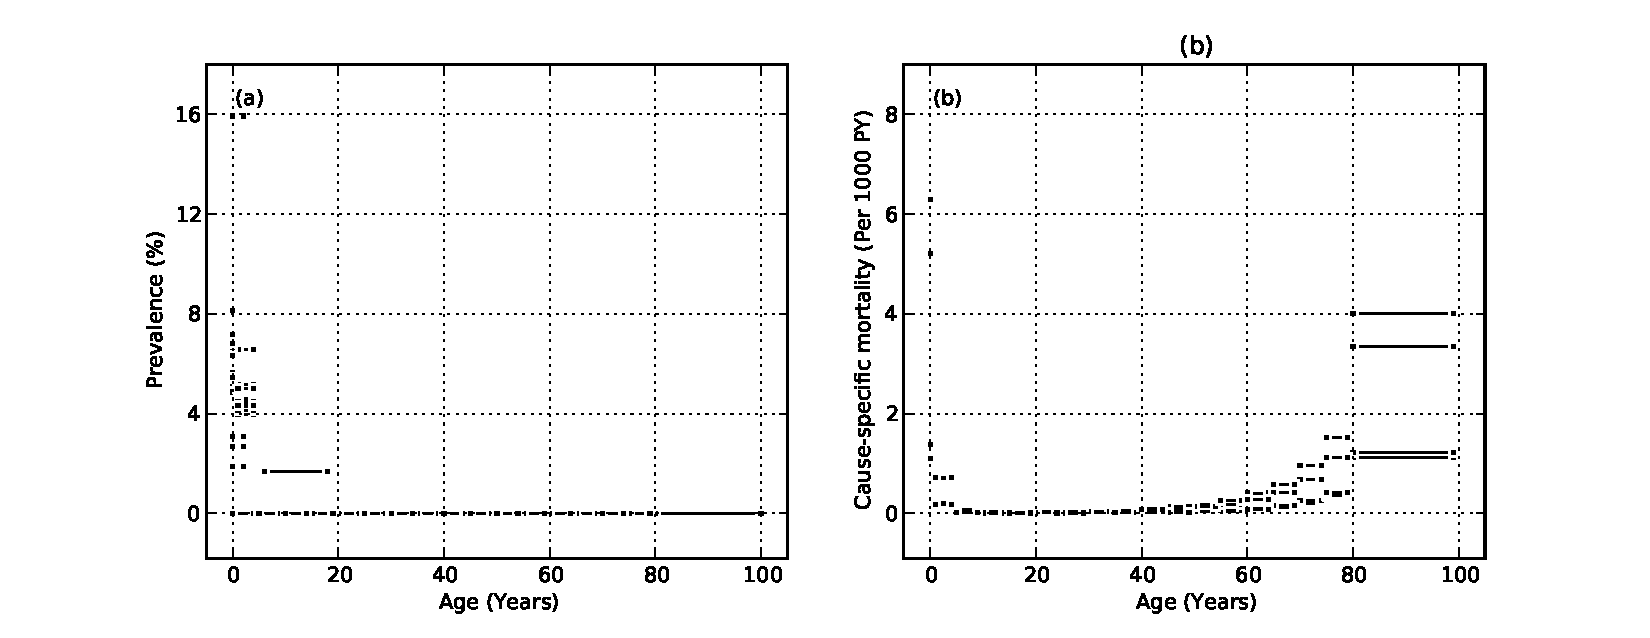
\includegraphics[width=\textwidth]{diarrhea-data.pdf}
            \caption{Diarrheal point prevalence (panel (a)) and
              cause-specific mortality (panel (b)) data in Central
              Latin America.}
            \label{fig:app-diarrhea data}
        \end{center}
    \end{figure}

Diarrheal diseases use a compartmental model to model all
epidemiological parameters for a single time, place and sex.  A
compartmental model estimates all epidemiological parameters
simultaneously which maintains internally consistent results as
discussed in Chapters \ref{sys-dynamics} and
\ref{applications-fits_incon_v_con}.  In addition to the systematic
review data, informative priors on the duration of diarrheal diseases
help guide the modeling process.  The prior for duration is set as the
prior for remission.  Duration priors produce less stable estimates
than the more directly parameterized remission priors.  Therefore
remission is the more appropriate prior for the model.  With the
assumption that the mortality hazard is low, Equation
\ref{eq:remission-duration} approximates the relationship between
duration and remission
    \begin{equation} \label{eq:remission-duration}
    	h_{r} = \frac{1}{h_{d}}
    \end{equation}
where $h_{r}$ is the epidemiological rate for remission and $h_{d}$ is
the epidemiological rate for duration in years.  Similar to the
discussion of priors in Chapter \ref{applications-con_fit_splines},
the choice of priors affects the epidemiological estimates.  However,
because of the logical requirement of internal consistency, a change
in the duration of diarrheal diseases has effects on all
epidemiological parameters as seen in Figure \ref{fig:app-diarrhea
  duration}.

    \begin{figure}[h]
        \begin{center}
            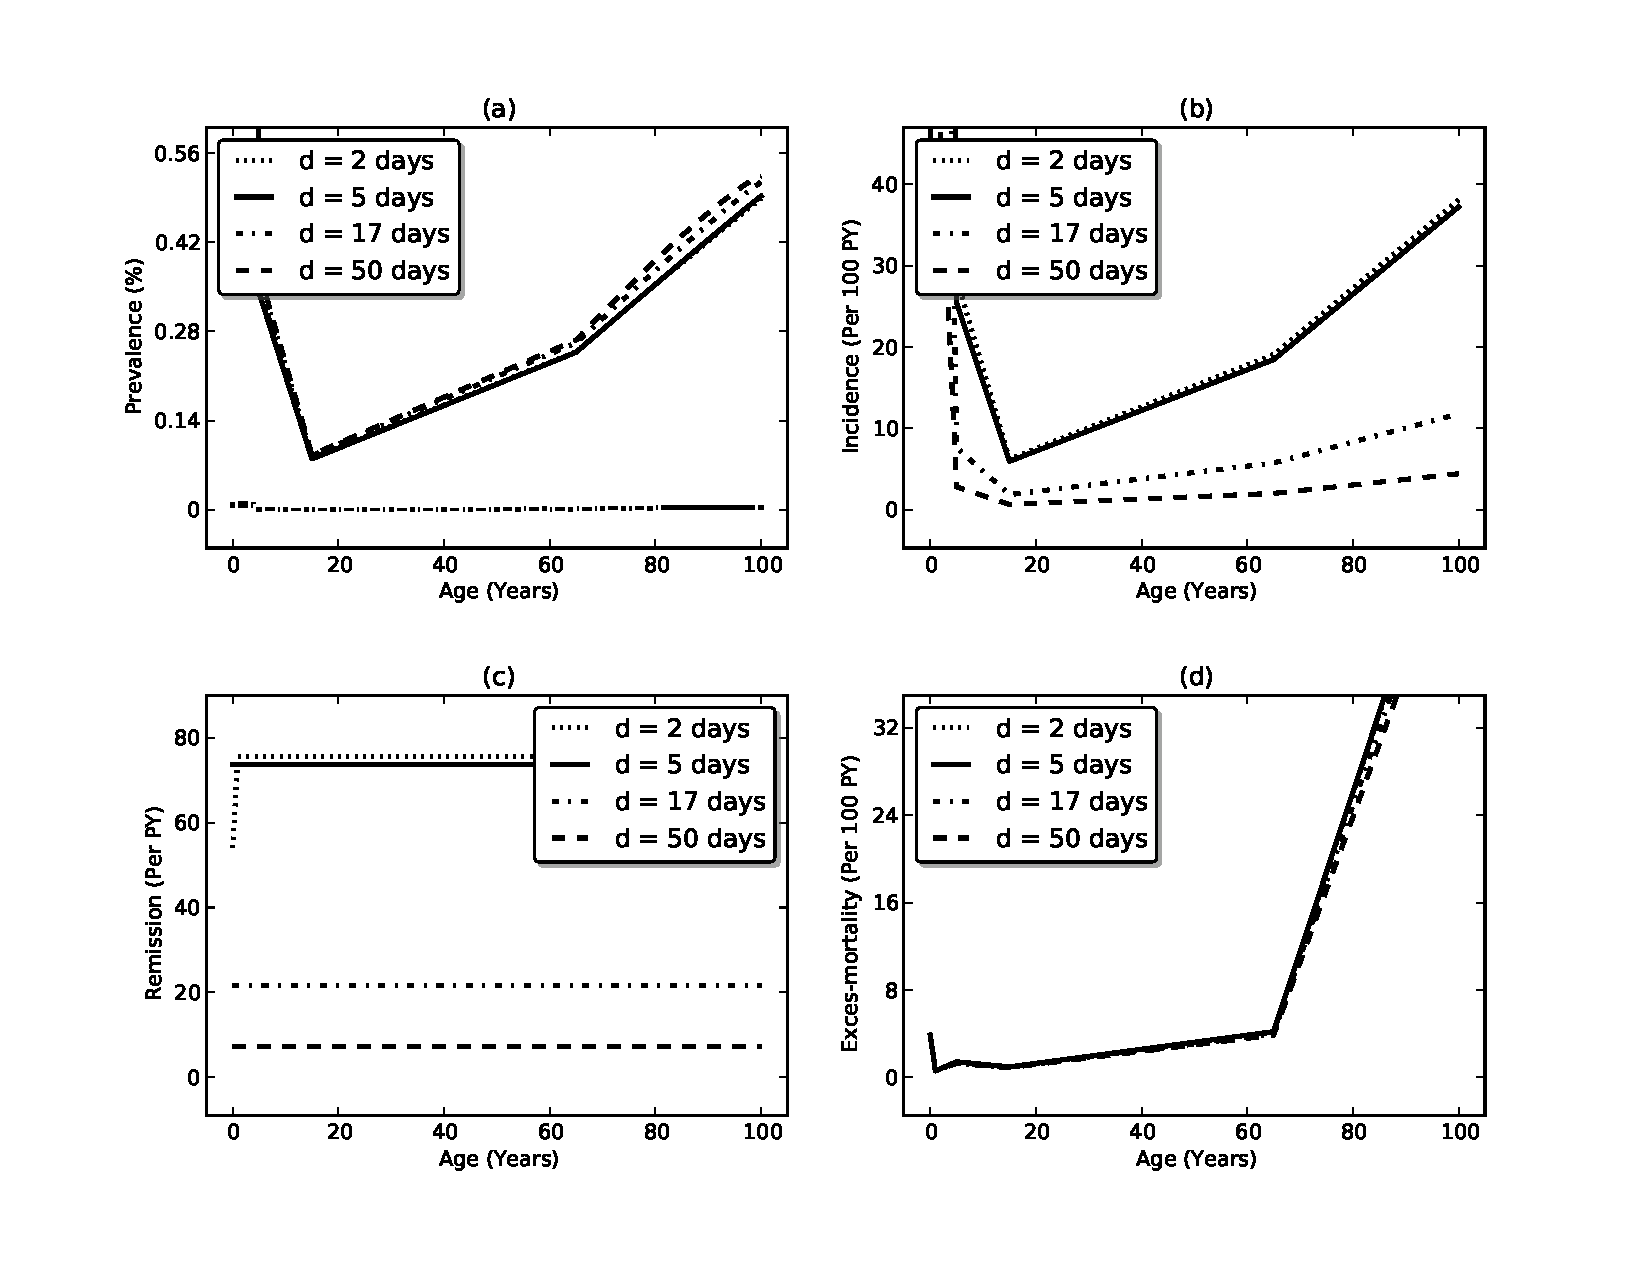
\includegraphics[width=\textwidth]{diarrhea-duration.pdf}
            \caption{Estimates of prevalence (panel (a)), incidence
              (panel (b)), remission (panel (c)) and excess-mortality
              (panel (d)) for diarrheal diseases in Central Latin
              American males in 2005 using a compartmental model with
              differing priors on disease duration, $d$.}
            \label{fig:app-diarrhea duration}
        \end{center}
    \end{figure}
